\newpage
\begin{tcolorbox}
	
	\lettrine{W}{ith} the rescue encroaching on the last days of expedition pushing, by the time we had  brought out all the kit from the cave, it was necessary to derig Primadona, and look back at what we had achieved.

 	In one wave, we reached the bottom of \emph{Upside Down} chamber and poked at the very final boulder choke, where water seeped through unstable boulders and impenetrable cracks. With no way on, we took the metal and ropes out of the low, wet pitches of our newly discovered series, and proceeded to put the cave to sleep. The entrance series ropes were brought up the pitches, but left in the cave.

	A couple of days later, it was time to pack up the bivi, store food safely, clean the metal work and stash the equipment we would leave on the mountain and take down the tents for the final descent to Ravne. We enjoyed the usual afternoon cheese cake with the Koblu{\v{c}}ar family with a refreshing lemon flavoured {\v{z}}ganje.

	The main outcome of this expedition to Primadona was the exposure of all that took part to bolting and rigging mainly vertical sections of cave, a departure from the format of previous years. For the leaders, there was ample opportunity to polish bolt placement and rigging skills and instil good practice in the younger generations. Expedition novices surveyed and rigged, but also gained many other communal living skills.

	It became obvious, after four weeks of systematic exploration that we had barely begun to scratch the surface in terms of cave development potential…
	\\
	\\
	\\
\end{tcolorbox}

	\backgroundsetup{	scale=1,
					color=black,
					opacity=1,
					angle=90,
					contents={%
 							 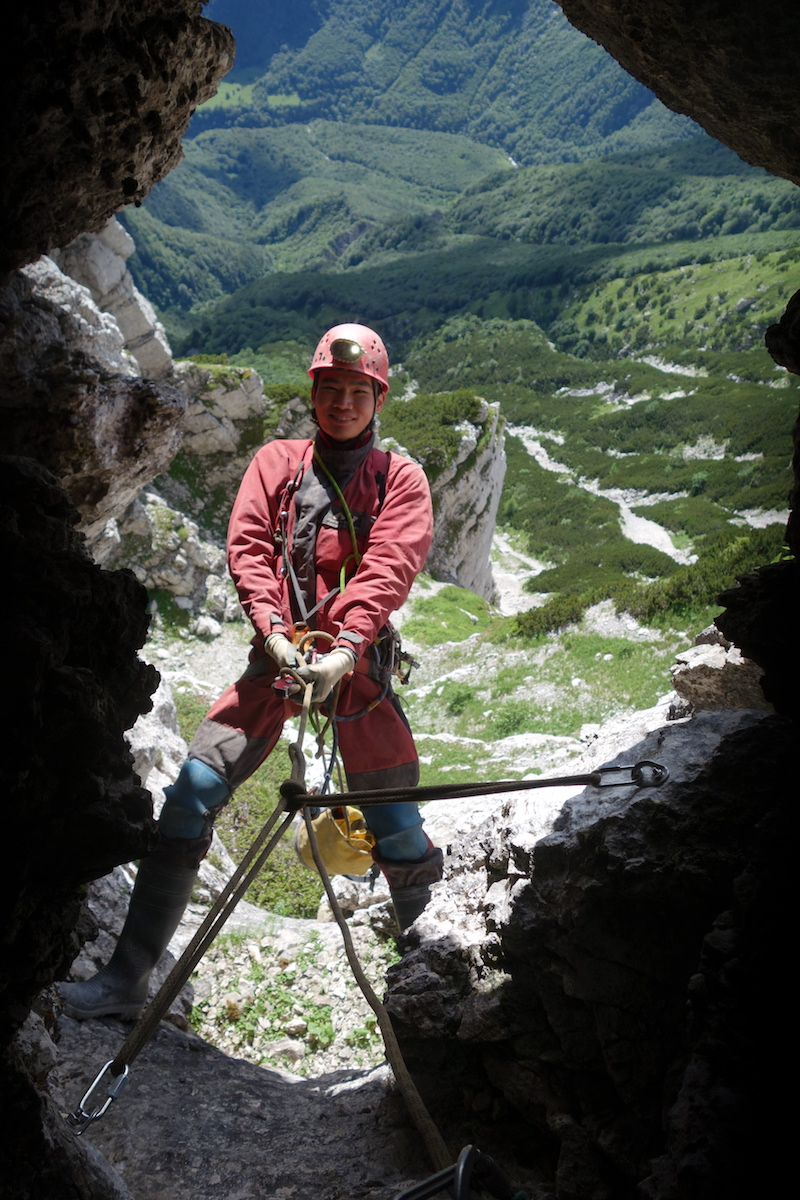
\includegraphics[width=\paperwidth, angle=270]{backgrounds/KennethB9.jpg}
 					}
	}
  
\BgThispage

